\documentclass[11pt]{article}

\usepackage{hyperref}
\usepackage{url}

\usepackage{algorithm}
\usepackage[noend]{algorithmic}

\usepackage{amssymb, amsmath}
\usepackage{graphicx}
\usepackage{comment}
\usepackage{enumitem}

\usepackage{geometry}
\geometry{left=1in,
          right=2in,
          top=1in,
          bottom=1in
          }

\newcommand{\RR}{\ensuremath{\mathbb{R}}}
\newcommand{\T}{\ensuremath{\top}}
\DeclareMathOperator{\diag}{diag}

\renewcommand{\leq}{\leqslant}
\renewcommand{\geq}{\geqslant}

\newcommand{\glad}{\textsc{glad}}
\newcommand{\tightglad}{\textsc{g\hspace{-1pt}l\hspace{-1pt}a\hspace{-1pt}d}}
\newcommand{\node}{\texttt{n}}
\newcommand{\parent}{\texttt{par}}
\newcommand{\anc}{\texttt{anc}}
\newcommand{\ch}{\texttt{ch}}
\newcommand{\SUBD}{\text{SUBD}}
\newcommand{\A}{\mathcal{A}}
\newcommand{\Ap}{\mathcal{A}^\prime}

\newcommand{\fix}{\marginpar{FIX}}
\newcommand{\new}{\marginpar{NEW}}

\title{A Scalable Deterministic Global Optimization Algorithm for Sparse Mixed Membership Matrix Factorization}

\author{
  Fan Zhang\\
  \texttt{fzhang@wpi.edu}
  \and
  Chauncey Wang\\
  \texttt{}
  \and
  Hachem Saddiki\\
  \texttt{hsaddiki@wpi.edu}
  \and
  Andrew Trapp\\
  \texttt{atrapp@wpi.edu}
  \and
  Patrick Flaherty\\
  \texttt{pjflaherty@wpi.edu}
}
\begin{document}

\maketitle

\begin{abstract}
Mixed membership models are popular for analyzing data sets that have within-sample heterogeneity. 
Several sampling and variational inference algorithms have been developed for mixed membership models, but they only provide approximate, locally optimal estimates. 
We use Benders' decomposition and the Global OPtimization (GOP) framework to derive an alternating algorithm that provides a guaranteed $\epsilon$-global optimum to a particular sparse mixed membership matrix factorization problem. 
Empirical results show that GOP is able to identify the global optima where iterated conditional modes (MAP), variational EM, and Metropolis-Hastings (MCMC) achieve only local optima even with multiple random initializations.
We derive a GOP inference algorithm is embarrassingly parallel in key optimization steps allowing the algorithm to scale nearly linearly with the size of the data set.
Finally, we show how the GOP framework can be easily extended to achieve globally optimal maximum a-posteriori estimates in general hierarchical Bayesian latent variable models.
\end{abstract}

\section{Introduction}\label{sec:intro}

Mixed-membership models have been used in document topic modeling \cite{Blei2003a}, collaborative filtering \cite{Mackey2010}, population genetics \cite{Pritchard2000}, and social network analysis~\cite{Airoldi:2008wi}. 
Such models account for data where an observed feature for a given sample is a mixture of shared, underlying groups. 
These groups are called topics in document modeling, subpopulations in population genetics, and communities in social network analysis. 
In bioinformatics applications the groups are called subtypes and we adopt that terminology here. 
Inference in mixed-membership models simultaneously identifies both the underlying subtypes and the distribution over those subtypes for each individual sample.

\subsection{Molecular Subtypes in Cancer}
Recently, it has become evident that many solid tumor samples are a heterogeneous mixture of genetic subtypes~\cite{Gerlinger:2012fs}. 
The heterogeneity is due to the presence of normal and immune cells in the biopsy as well as multiple genetic subtypes in the cancer tissue~\cite{}. 
The measured expression level for a gene in a sample is then a convex weighted combination of the expression level in each cellular subpopulation where the weights are the fraction of that subpopulation in the sample.


However, most tumor classification methods for cancer subtyping make an all-or-none assumption~\cite{}. 
This assumption and subsequent treatment decision can lead to mono-therapy treatment failure because a potentially sizable fraction of the tumor is left untreated by focusing therapeutic effort on the majority subtype~\cite{}. 
Therefore, there is a need for a mixed-membership model to accurately estimate the tumor subtype distribution in heterogeneous tumor samples.

\subsection{Mixed Membership Models}
% Model structure
Continuous mixed membership statistical models have a latent Dirichlet random variable that allows each sample to have its own distribution over subtypes and a latent variable for the feature weights that describe each subtype. 
The inferential goal is to estimate the joint posterior distribution over these latent variables and thus obtain the distribution over subtypes for each sample and the feature vector for each subtype.

Sampling or variational inference methods are commonly used to estimate the posterior distribution of interest. 
A mean-field variational algorithm~\cite{Blei2003a} and a collapsed Gibbs sampling algorithm have been developed for Latent Dirichlet Allocation~\cite{Xiao2010}. 
Alternatively, inference may be viewed as a particular matrix factorization problem~\cite{Mackey2010}.


There is a tight connection between mixed membership models
and matrix factorization~\cite{Singh2008}. Non-negative
matrix factorization techniques have been used in image
analysis and collaborative filtering applications
\cite{Lee1999,Mackey2010}. Topic models for document clustering have been cast as a matrix factorization problem~\cite{Xu2003}.

The basic mixed membership model structure has been extended
in various interesting ways. A hierarchical Dirichlet prior
allows one to obtain a posterior distribution over the number
of subtypes~\cite{Teh2005}. A prior on the subtype variables
allows one to impose specific sparsity constraints on the
subtypes~\cite{Kaban:2007gz,MacKay:1992ul,Taddy:2012dd}.
Correlated information may be incorporated to improve the
coherence of the subtypes~\cite{Blei2006}.

\subsection{Deterministic Global OPtimization (GOP)}
In many applications it is important to obtain the globally optimal solution rather than a local or approximate solution. 
Recently there have been significant advances in deterministic optimization methods for general nonconvex optimization problems~\cite{Floudas2008, Horst2002}. 
Deterministic strategies include: covering methods, branch and bound methods, cutting plane methods, interval methods and others. 
Here, we build on Benders' decomposition and GOP to develop a cutting plane method to solve for the global optimal solution for mixed membership matrix factorization.


\subsubsection{Benders' Decomposition}

% Discuss global optimization methods broadly
Benders' decomposition provides a way to separate the decision variables in an optimization problem in such a way that alternating between solving two optimization problems over the subsets of variables yields a global optimum \cite{Benders1962,Geoffrion1972}. So-called ``complicating variables'' -- variables that when temporarily held fixed render the optimization problem more tractable -- are separated from other variables. 
Alternating between the two optimization problems involving both sets of variables yields an algorithm that converges to the global optimum. 
However, Benders' decomposition was originally limited to situations where the subproblem was a linear program~\cite{Benders1962}.


\subsubsection{Global OPtimization Overview}

The Global OPtimization (GOP) approach is a recent adaptation of Benders' decomposition that minimizes computational complexity of the alternating algorithm while providing an $\epsilon$-global to a more general class of problems that includes mixed-integer biconvex optimization problems~\cite{Floudas1990}. 

\subsubsection{Global OPtimization Problem Conditions}

\subsubsection{Cutting Plane Algorithm for Global OPtimization}

\subsubsection{Branch-and-Bound Algorithm for Global OPtimization}


\section{Problem Statement}\label{sec:problem} 

The problem data is a matrix $y \in \RR^{M \times N}$, where an element $y_{ji}$ is an observation of feature $j$ in sample $i$. 
We would like to represent each column of $y$ as $y_i = x \theta_i$, where $x \in \RR^{M \times K}$ is a matrix of $K$ subtype vectors and $\theta_i \in\Delta^{K-1}$ is the $i$th sample's distribution over the $K$ subtypes. 
We would like $x$ to be sparse because doing so makes interpreting the subtypes easier and often $x$ is believed to be sparse a-priori for many interesting problems. 
In the specific case of cancer subtyping, $y_{ji}$ may be a normalized gene expression measurement for gene $j$ in sample $i$. 
We write this matrix factorization problem as

\begin{flalign}\label{eqn:opt1}
	\underset{\theta,x}{\text{minimize}}  &\  \|y_i-x\theta_i\|^2_2 \nonumber\\
	\text{subject to} &\  \|x\|_1 \leq P \\
	&\  \theta_i \in \Delta^{K-1}\  \forall i. \nonumber
\end{flalign}

Optimization problem~\eqref{eqn:opt1} can be recast with a biconvex objective and a convex domain as
\begin{flalign}\label{eqn:opt2}
	\underset{\theta,x,z}{\text{minimize}}      &\  	\|y-x\theta\|^2_2 \nonumber\\
	\text{subject to}   &\  \sum_{j=1}^M \sum_{k=1}^K z_{jk} \leq P \\
                    &\  -z_{jk} \leq x_{jk} \leq z_{jk} \ \forall j,k \nonumber\\
                    &\  \theta_i \in \Delta^{K-1}\  \forall i, z_{jk} \geq 0\  \forall (j,k).\nonumber
\end{flalign}

If either $x$ or $\theta$ is known then \eqref{eqn:opt2} reduces to a convex optimization problem. 
Indeed, if $x$ is fixed, the optimization problem is a form of constrained linear regression. 
If $\theta$ is fixed, we have a form of LASSO regression.

%A common approach for solving an optimization problem with a biconvex objective function is to alternate between fixing one variable and optimizing over the other. 
%However, this approach only provides a local optimum~\cite{Gorski2007a}.


\section{Approach}\label{sec:approach}

We use the Global OPtimization (GOP) approach to solve for $\epsilon$-global optimum values of $x$ and $\theta$~\cite{Floudas1990,Floudas1994}. 



An overview of the GOP inference algorithm for GLAD is outlined in Algorithm~\ref{alg:gop1}.

\begin{algorithm}[h]
\caption{GLAD-GOP Inference Algorithm Overview}
\label{alg:gop1}

\begin{algorithmic}[1]
\STATE partition the optimization problem variables into the relaxed master problem and the subproblem
\STATE initialize relaxed master problem branch-and-bound tree root node

\REPEAT
\STATE solve the subproblem at the current node

\STATE accumulate the active qualifying constraints from the current node and all its ancestor nodes

\STATE collect the set of unique regions defined by the current node subproblem optimal dual variables

\FOR{each unique region defined by the qualifying constraints from the current node subproblem solution}

\STATE create a leaf and populate it with the solution of a relaxed master problem defined by the qualifying constraints in the node and all of its ancestors

\ENDFOR

\STATE jump to the branch-and-bound tree leaf with the smallest relaxed master problem solution
\UNTIL{upper bound - lower bound $< \epsilon$}

\end{algorithmic}
\end{algorithm}
Note that each relaxed master problem can be solved independently and so these problems can be solved in parallel.

The relaxed master problem branch-and-bound tree holds information from the current and relevant previous iterations of the GOP inference algorithm.
A node in the tree contains: 
\begin{itemize}[noitemsep]
\item qualifying constraints that define a unique region in $\mathcal{X}$;
\item $x^*$, the optimizing value of the relaxed master problem with constraints given by the current node and all its ancestors;
\item $Q*$, the optimal value of the relaxed master problem; and
\item $\lambda^*$ and $\mu^*$ the optimal dual variables from the subproblem optimized at the parent node's value of $x$.
\end{itemize}

\subsection{Partition the Optimization Problem into the Relaxed Master Problem and the Subproblem}
We start by partitioning the problem into a relaxed master problem and subproblem. The variable $Q$ is used later to enforce the Lagrange function constraints passed from the subproblem to the master problem; these constraints implicitly represent subproblem information in a compact manner.

\noindent\fbox{
\begin{minipage}[c][16em][t]{1\textwidth}
\centering
  \textbf{Relaxed Master Problem} \\
  ($\theta$ fixed)
    \begin{flalign*}
    \underset{Q,x,z}{\text{minimize}}     &\  Q \\
    \text{subject to}   &\  \sum_{j=1}^M \sum_{k=1}^K    z_{jk} \leq P \\ 
                        &\  -z_{jk} \leq x_{jk} \leq z_{jk},\  z_{jk} \geq 0\\
						& \text{for}\  t \in \{ \anc(\node(T)), \node(T)\}
						\begin{cases}
						Q \geq L(x,\theta^{B}(t), y, \lambda^{t},\mu^{t})\big\vert^{\text{lin}}_{x^{t}, \theta^{t}} \\
						g^{t}_{ki}\big\vert^{\text{lin}}_{x^{t}}(x) \leq 0\  \text{if}\  \theta^{B}(t)_{ki} = 1\\
						g^{t}_{ki}\big\vert^{\text{lin}}_{x^{t}}(x) \geq 0\  \text{if}\  \theta^{B}(t)_{ki} = 0
						\end{cases}
\end{flalign*}
\end{minipage}%
}

\noindent\fbox{
\begin{minipage}[c][9em][t]{1\textwidth}
\centering
  \textbf{Subproblem} \\
  ($x$ fixed)
%  	\vspace{3em}
    \begin{flalign*}
    \underset{\theta}{\text{minimize}}     &\  \|y-x\theta\|^2_2 \\
    \text{subject to}   &\  \theta_i^T 1_K = 1 \\
                    &\  \theta_{ki} \geq 0 
    \end{flalign*}
\end{minipage}%
}

\subsection{Initialize the relaxed master problem branch-and-bound root tree node}

GOP iterations are started by creating a root node with randomly initialized master problem decision variables, $x^{(0)}$ and optimal relaxed master problem objective function value $Q=-\infty$.
The iteration counter $T$ is then set to $T=1$ and the algorithm begins alternating between the subproblem and master problem.
The algorithm jumps between leaf nodes in the branch-and-bound tree at each iteration, so we denote the current branch-and-bound tree node at iteration $T$ as $\node(T)$. The parent of $\node(T)$ is denoted $\parent(\node(T))$, the set of ancestors of $\node(T)$ is denoted $\texttt{an}(\texttt{n}(T))$, and the set of children of $\texttt{n}(T)$ is denoted $\texttt{ch}(\texttt{n}(T))$.

\subsection{Solve subproblem with the current node relaxed master problem decision variables}

The subproblem for the current node at iteration $T$, $\node(T)$, is solved with fixed relaxed master problem decision variables, $x^{(\node(T))}$. 
The solution provides optimal dual Lagrange variables $\lambda^{(\node(T))}$ and $\mu^{(\node(T))}$ for the equality and inequality constraints.
The global upper bound, $\SUBD$, is updated with the subproblem optimal value, $S^{(\node(T))}$, according to $\SUBD \leftarrow \min\{\SUBD, S^{(\node(T))} \}$.

\subsection{Accumulate the active qualifying constraints from the current node and all its ancestor nodes}

Information is passed from the subproblem to the relaxed master problem through the subproblem Lagrange function, $L$ and associated \emph{qualifying constraints}, $g$ which are both functions of the optimal subproblem dual variables. 
By construction, all of the qualifying constraints in $\anc(\node(T))$ and $\node(T)$ are satisfied at $x^{\node(T)}$. 
These active qualifying constraints are accumulated to form the set $QC(\node(T))$.
The set qualifying constraints from each ancestor node defines a region in $\mathcal{X}$ and the Lagrange function $L$ defines a lower bound on the relaxed master problem objective.
Therefore, the domain of the relaxed master problem shrinks at each level of the branch-and-bound tree and lower bound on the objective increases at each level of the tree.
The relaxed master problem becomes progressively less relaxed.


\subsection{Collect the set of unique regions defined by the current node subproblem optimal dual variables}

Every qualifying constraint defined from the optimal Lagrange dual function of the subproblem at node $\node(T)$ defines a hyperplane or ``cut'' in $\mathcal{X} \in \RR^{MK}$.
A leaf node below the current node is constructed for each unique region defined by the hyperplane arrangement.
There are $KN$ hyperplanes because in the GOP framework we have one hyperplane for each so-called ``connected variable'' and all of the $KN$ elements of $\theta$ are connected variables.
So, an upper bound on the number of regions defined by $KN$ cuts is $2^{KN}$ because each region may be found by selecting a side of each cut.
Indeed, the GOP Cutting Plane Algorithm solves a relaxed master problem for each of the $2^{KN}$ possible regions.
While the cutting plane algorithm is guaranteed to test every region and thus achieve the global optimum, it is inefficient because it considers many cases that result in a vacuous region.

A set of hyperplanes is called an arrangement, $\A$, and the set of unique regions defined by $\A$ is $r(\mathcal{A})$.
In our particular situation, all of the hyperplanes pass through the unique point $x^{(\node(T))}$, so all of the regions are unbounded except by the constraints provided in $\mathcal{X}$.
Thomas Zaslavsky, in his 1973 PhD Thesis, provided a recursive algorithm for counting the number of regions $|r(\A)|$.
Indeed, $|r(\A)|$ is often much less that $2^{|\A|}$.
However, due to its recursive nature, computing the number of hyperplanes using Zaslavsky's theorem is computationally slow.
So, we have developed an A-star search algorithm to simultaneously count and identify the set of unique regions defined by arrangement $\A$.

First, we preprocess the arrangement $\A$ to eliminate trivial and redundant hyperplanes.
We eliminate a hyperplane from $\A$ if the coefficients are all zero.
We also eliminate duplicate hyperplanes in $\A$ if two hyperplanes are such that
%TODO: add tolerance formula here
\begin{equation*}
XXX
\end{equation*}
We are left with a reduced arrangement, $\A^\prime$.

We define $\theta^{B} \in \{0,1\}^{|r(\Ap)| \times KN}$. 
The $b$-th region in $r(\Ap)$ is uniquely identified by the zero-one vector in the $b$-th row of $\theta^{B}$.
If the $b$-th element of the $ki$-th row of $\theta^{B}$ is $+1$, then $g_{ki} \leq 0$.
Similarly, if the $b$-th element of the $ki$-th row of $\theta^{B}$ is $0$, then $g_{ki} \geq 0$.

The A-star search algorithm completes the $\theta^{B}$ matrix for the current node $\node(T)$ and a leaf node is generated for each row of $\theta^{B}$.
Thus each unique region defined by the qualifying constraint cuts provided by the Lagrange dual of the subproblem at the current node.
%TODO describe A-star search algorithm here

\subsection{Create a leaf and populate it with the solution of a relaxed master problem defined by the qualifying constraints in the node and all of its ancestors}

A unique region in $\mathcal{X}$ for the leaf node $\texttt{ch}(\texttt{n}(T))$ is defined by the $b$-th row of $\theta^{B}$ derived from the subproblem at node $\node(T)$.
We can write this region as the qualifying constraint set,
\begin{align*}
g^{\ch(\node(T))}_{ki}\big\vert^{\text{lin}}_{x^{\node(T)}}(x) \leq 0\  \text{if}\  \theta^{B}(b)_{ki} = 1\\
g^{\ch(\node(T))}_{ki}\big\vert^{\text{lin}}_{x^{\node(T)}}(x) \geq 0\  \text{if}\  \theta^{B}(b)_{ki} = 0
\end{align*}

We create the $b$-th child node of $\node(T)$ and populate it with this constraint set and $\theta^{B}(b)$ which will be used in the construction of the Lagrange function lower bound in the relaxed master problem.

Now, we construct and solve the relaxed master problem at $\ch(\node(T))$. 
First, we add the qualifying constraint sets contained in each node along the path in the branch-and-bound tree from $\ch(\node(T))$ to the root inclusively.
For example, the qualifying constraint set for a node $\node^\prime$ along the path is
\begin{align*}
g^{\node^\prime}_{ki}\big\vert^{\text{lin}}_{x^{\node^\prime}}(x) \leq 0\  \text{if}\  \theta^{B}(\node^\prime)_{ki} = 1\\
g^{\node^\prime}_{ki}\big\vert^{\text{lin}}_{x^{\node^\prime}}(x) \geq 0\  \text{if}\  \theta^{B}(\node^\prime)_{ki} = 0,
\end{align*}
where $g^{\node^\prime}_{ki}$ is the node's $ki$-th qualifying constraint, $x^{\node^\prime}$ is the node's relaxed master problem optimizer, and $\theta^{B}(\node^\prime)$ is the $0-1$ vector defining the unique region for node $\node^\prime$.

Second, we add the Lagrange function lower bound constraints constructed from each node along the path in the branch-and-bound tree from $\ch(\node(T))$ to the root inclusively.
For example,
\begin{equation*}
L(x,\theta^{B}(\node^\prime), y, \lambda^{(\node^\prime)},\mu^{(\node^\prime)})\big\vert^{\text{lin}}_{x^{(\node^\prime)}, \theta^{(\node^\prime)}},
\end{equation*}
where XXX.

We finish the relaxed master problem construction by adding the remaining constraints and objective function outlined in Section~\ref{}.

The resulting relaxed master problem is a linear program and can be solved efficiently using gurobi.
We store the optimal value and the optimizing decision variables in the node.
Once a relaxed master problem has been solved for each leaf of the current node at iteration T, $\node(T)$, we move to the final step of the iteration -- selecting the lowest lower bound provided by all of the leaf node relaxed master problem solutions.


\subsection{Jump to the branch-and-bound tree leaf with the smallest relaxed master problem solution}

We maintain a dictionary where the value of a record is a pointer to a branch-and-bound tree node and the key is the optimal value of the relaxed master problem at that leaf node.
Using this dictionary, we select the smallest key and jump to the node of the tree indicated by the value.
We eliminate that element from the dictionary since at the end of the next iteration, it will be an interior node and not available for consideration.
We increment the iteration count $T \leftarrow T+1$ and we update the GOP lower bound $MLBD \leftarrow f(x)$.

Since we always select the lowest lower bound provided by the relaxed master problem, the lower bound is non-decreasing.
If our convergenece criteria $SUBD - MLBD \leq \epsilon$ has been met, then we exit the algorithm and report the optimal $\theta$ from the node's subproblem and the optimal $x$ from the node's relaxed master problem.



We briefly provide derivations for the Lagrange function and the qualifying constraints here. 
First, the Lagrange function for the subproblem is 
\begin{equation}\label{eqn:lagrange1}
    \begin{split}
    L(x, \theta, \lambda, \mu) &= \sum_{i=1}^N L(x, \theta_i, \lambda_i, \mu_i)\\
    &= \sum_{i=1}^N (y_i - x \theta_i)^\T (y_i - x\theta_i) - \lambda_i (\theta_i^\T 1_K - 1) - \mu_i^\T \theta_i\\
    &= \sum_{i=1}^N y_i^\T y_i -2 y_i^\T x \theta_i + \theta_i^\T x^\T x \theta_i - \lambda_i (\theta_i^\T 1_K - 1) - \mu_i^\T \theta_i
    \end{split}
\end{equation}
where $\mu \in \RR_+^{K \times N}$ and $\lambda \in \RR^N$.

The relaxed master problem makes use of the Lagrange function linearized about $\theta^{(t)}$ which we obtain with a Taylor series approximation,
\begin{equation}
    L(x, \theta_i, \lambda_i, \mu_i) \big\vert_{\theta^{(t)}}^{\text{lin}} \triangleq L(x, \theta_i^{(t)}, \lambda_i^{(t)}, \mu_i^{(t)}) + \sum_{k=1}^K g_{ki}^{(t)}(x) \cdot \left(\theta_{ki} - \theta_{ki}^{(t)} \right),
\end{equation}
where 
\begin{equation}\label{eqn:qc1}
g^{(t)}_{i}(x) \triangleq \nabla_{\theta_i} L \left(\theta_i, x, \lambda_i^{(t)}, \mu_i^{(t)} \right) \big\vert_{\theta_i^{(t)}} = -2 y_i^\T x + 2 \theta^{(t)\T}_i x^\T x - 1_K^\T \lambda_i^{(k)} - \mu_i^{(k)\T}.
\end{equation}

The qualifying constraint is quadratic in $x$. However, we require it to be linear in $x$ to yield a convex domain if $g^{(t)}_{i}(x) \geq 0$ or $g^{(t)}_{i}(x) \leq 0$. 
So, we linearize the Lagrangian first with respect to $x$ about $x^{(t)}$ then about $\theta_i$ at $\theta_i^{(t)}$. 
While the linearized Lagrangian is not a lower bound everywhere in $x$, it is a valid lower bound in the region bound by the qualifying constraints with $\theta_i$ set at the corresponding bounds in the Lagrange function.

The Lagrange function linearized about $x^{(t)}$ is
\begin{equation}
L(y_i, \theta_i, x, \lambda_i, \mu_i) \bigg\vert^{\text{lin}}_{x^{(t)}} \triangleq 
y_i^T y_i - \theta_i^\T x^{(t)\T} x^{(t)} \theta_i - 2 y_i^\T x \theta_i + 2 \theta_i^\T x^{(t)\T} x \theta_i - \lambda_i(\theta_i^\T 1_K - 1) - \mu_i^\T \theta_i.
\end{equation}

Now, the Lagrange function linearized about $(x^{(t)}, \theta_i^{(t)})$ is
%
\begin{equation}
\begin{split}
L(y_i, \theta_i, x, \lambda_i, \mu_i) \bigg|^{\text{lin}}_{x^{(t)}, \theta_i^{(t)}} \triangleq\ & y_i^\T y_i + \theta_i^{(t)\T} x^{(t)\T} x^{(t)} \theta_i^{(t)} -2 \theta_i^{(t)\T} x^{(t)\T} x^{(t)} \theta_i \\
& - \lambda_i(1_K^\T \theta_i - 1) - \mu_i^\T \theta_i \\
& - 2 \theta_i^{(t)\T} x^\T x^{(t)} \theta_i^{(t)\T} - 2 y_i^\T x \theta_i + 2 \theta_i^{(t)\T} (x^{(t)\T} x + x^\T x^{(t)}) \theta_i
\end{split},
\end{equation}
%
and the gradient used in the qualifying constraint is
%
\begin{equation}
	\begin{split}
		g^{(t)}_i\big\vert^{\text{lin}}_{x^{(t)}}(x) &\triangleq \nabla_{\theta_i} \left[ L(y_i, \theta_i, x, \lambda_i, \mu_i) \bigg|^{\text{lin}}_{x_0} \right] \bigg|_{\theta_i^{(t)}} \\
		& = -2 x^{(t)\T} x^{(t)} \theta_i^{(t)} -2 x^\T y_i + 2 (x^{(t)\T} x + x^\T x^{(t)}) \theta_i^{(t)} - \lambda_i 1_K - \mu_i.
\end{split}
\end{equation}

Once the valid qualifying constraints from the previous $t=1,\ldots,T-1$ iterations have been identified and incorporated, the constraint for the current $T$-th iteration is
%
\begin{eqnarray*}
Q \geq & L(x,\theta^{B_T}, y, \lambda^{(t)},\mu^{(t)})\big\vert^{\text{lin}}_{x^{(t)}, \theta^{(t)}}\\
&g_{ki}^{(T)}\big\vert^{\text{lin}}_{x^{(t)}}(x) \leq 0 \ \text{if}\ \theta^{B_T}_{ki} = 1 \\
&g_{ki}^{(T)}\big\vert^{\text{lin}}_{x^{(t)}}(x) \geq 0 \ \text{if}\ \theta^{B_T}_{ki} = 0.
\end{eqnarray*}
%
The master problem must be solved once for each possible setting of the subproblem variables at their bounds. 
In general, we only need to set the ``connected'' subproblem variables at their bounds, but the matrix factorization problem structure renders all $KN$ subproblem variables connected. 
Thus we have the computationally complex situation of needing to solve $2^{KN}$ relaxed master problems at each iteration. 
This is the price we pay for an exact solution.
However, as detailed later, there are several ways of reducing this computational burden.

All of the $2^{KN}$ solutions, $Q$, of the relaxed master problem are appended to a list at each iteration. 
The minimum $Q$ in this list is selected for the new global lower bound $\text{MLBD}$ and the optimal $x^{(T)}$ is updated to the corresponding optimizing decision variable. 
The solution is removed from the list so that it is not selected in a later iteration. 
If the lower and upper bounds are within the specified tolerance $\epsilon$, the algorithm terminates with the $\epsilon$-global optimum solution in $x^{(T)}$. 
Finite $\epsilon$-convergence and $\epsilon$-global optimality proofs are given in~\cite{Floudas1994}.


\section{Results}\label{sec:results}


\subsection{Illustrative Example}
%
We use a simple data set in order to show the
operation of the algorithm in detail and facilitate visualization of the cut sets. The data set, $y$, and true
decision variable values, $(x^*, \theta^*)$, are
%
\begin{eqnarray*}
	x^* =
	\left[ 
	\begin{array}{cc} 
		-1, & 0
	\end{array} 
	\right],
	&
	\theta^* = 
	\left[ 
	\begin{array}{ccc} 
		1, & 0, & 0.5 \\
		0, & 1, & 0.5
	\end{array} 
	\right],
	&
	y = 
	\left[ 
	\begin{array}{ccc} 
		-1, & 0, & -0.5
	\end{array} 
	\right].
\end{eqnarray*}
%
We ran the GOP algorithm with sparsity constraint variable $P=1$ and convergence tolerance $\epsilon = 0.01$. 
There are $KN = 6$ connected variables, so we solve $2^{KN} = 64$ relaxed master problems at each iteration. 
These relaxed master problems are independent and can be distributed to different computational threads or cores. 
The subproblem is a single optimization problem and need not be distributed. 
The optimal decision variables after 72 iterations are
%
\begin{eqnarray*}
	\hat{x} = x^{(72)} =
	\left[ 
	\begin{array}{cc} 
		-0.920, & 0.080
	\end{array} 
	\right],
	&
	\hat{\theta} = \theta^{(72)} =
	\left[ 
	\begin{array}{ccc} 
		1.00, & 0.080, & 0.580 \\
		0.00, & 0.920, & 0.420
	\end{array} 
	\right],
\end{eqnarray*}
%
and the Lagrange multipliers are $\hat{\lambda} = [-0.147, 0, 0]$ and $\hat{\mu} = [0, 0, 0; 0.160, 0, 0]$.

Figure~\ref{fig:figs_bounds_and_trace}A shows the convergence of the upper and lower bounds by iteration. 
The upper bound converges quickly and the majority of the time in the algorithm is spent proving optimality. 
With each iteration regions of the solution space are tested until the lower bound is tightened sufficiently to meet the stopping criterion. 
Figure~\ref{fig:figs_bounds_and_trace}B shows the first six $x$ values considered by the algorithm with isoclines of the objective function with $\theta^*$ fixed. 
It is evident that the algorithm is not performing hill-climbing or any other gradient ascent algorithm during its search for the global optimum. 
Instead, the algorithm explores a region bound by the qualifying constraints to construct a lower bound on the objective function. 
Furthermore, the algorithm does not search nested regions, but considers previously explored cut sets.

\begin{figure}[ht]
	\centering
		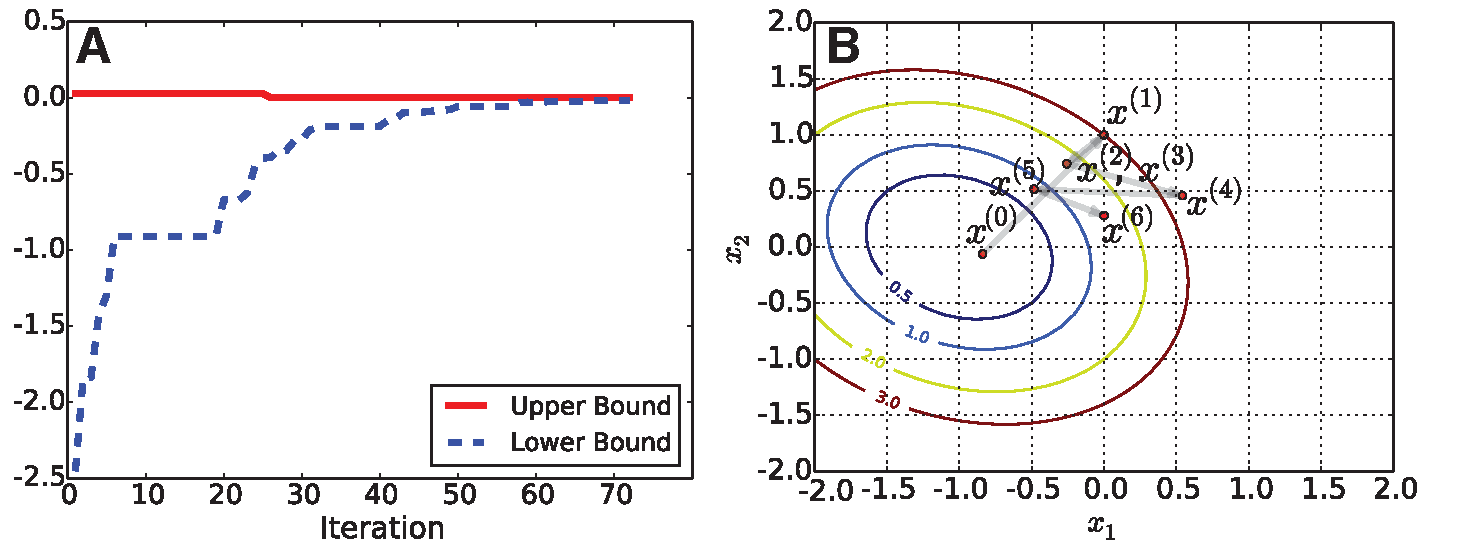
\includegraphics[width=1.0\textwidth]{figs/bounds_and_trace.pdf}
	\caption{(A) Upper and lower bounds converge to $\epsilon$-global optimal solution. (B) First six iterations of GOP algorithm in $x$ space with contours of the objective function at optimal $\theta^*$.}
	\label{fig:figs_bounds_and_trace}
\end{figure}

Figure~\ref{fig:figs_GOP_cutting_plane_sequence} shows the sequence of cut sets for the first three iterations of the algorithm. 
One cutting plane is obtained for each of the $KN$ qualifying constraints. 
We initialize the algorithm at $x^{(0)}$. 
The blue solid lines in the subfigure for the zero-th iteration show the cuts with $g^{(t)}_i\big\vert^{\text{lin}}_{x^{(t)}}(x) = 0$. The GOP algorithm solves $2^{KN}$ relaxed master
problems; to provide a lower bound in each region. 
The value of $x$ that yields the smallest lower bound is selected for the next iteration -- shown as $x^{(1)}$. 
Then $KN$ cuts are generated about $x^{(1)}$ (shown in the middle subfigure). 
The previous cuts are shown as dotted lines. Again $2^{KN}$ relaxed master problems are solved, but now the regions are the intersecton of the region containing $x^{(1)}$ from the previous iteration and all of the regions defined in the current iteration cut set. 
The $x$ that achieves the lowest lower bound is selected as $x^{(2)}$ and the algorithm continues incorporating the previous cut regions.

\begin{figure}[ht]
	\centering
		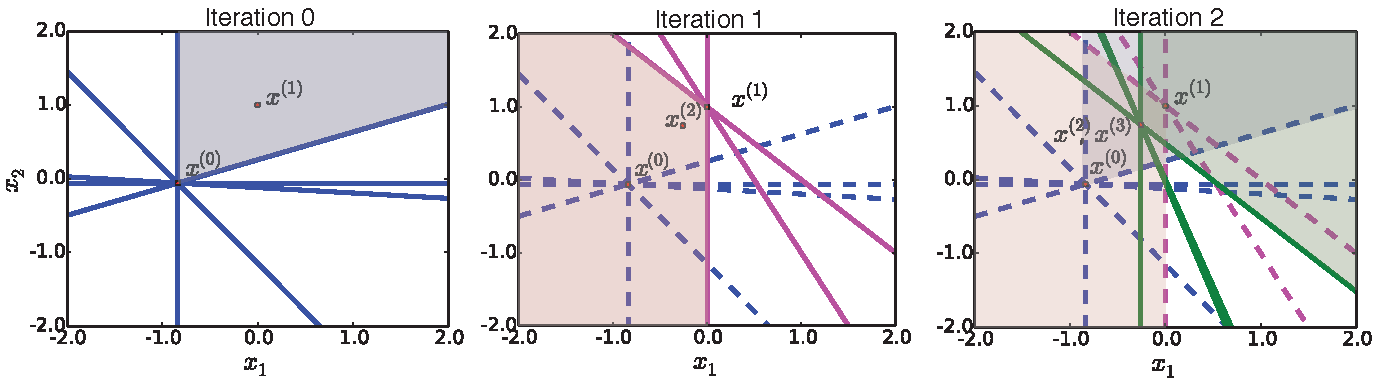
\includegraphics[width=1.0\textwidth]{figs/GOP_cutting_plane_sequence.pdf}
	\caption{Cut set regions for the first three iterations of the GOP algorithm for sparse mixed membership matrix factorization. Refinement of the relaxed master problem solution space and lower bound achieves $\epsilon$-global optimality.}
	\label{fig:figs_GOP_cutting_plane_sequence}
\end{figure}


\subsection{Comparison to inference algorithms}
%TODO Compare to ICM, variatonal EM, metropolis-hastings


\subsection{Computational Complexity}
%TODO Compare to cutting plane, branch-and-bound, MILP, without hyperplane caching, GLAD-GOP

\subsection{Genomic Subtypes in Breast Cancer Gene Expression Data}

\section{GOP for Hierarchical Models}\label{sec:stats}
%
The general scalar exponential family distribution function takes the form
\begin{equation}
	f_X(x|\eta) = h(x)\exp\left\{ \eta T(x) - A_X(\eta) \right\},
\end{equation}
where $\eta$ is the natural parameters, $T(x)$ is the sufficient statistic, $h(x)$ is the base measure, and $A(\eta)$ is the log-partition function.

Consider a hierarchical Bayesian model with a conjugate prior on $\eta$ with hyperparameters $\nu$,
\begin{equation}
	f_\eta(\eta|\nu) = h(\eta)\exp\left\{ \nu T(\eta) - A_\eta(\nu) \right\},
\end{equation}

The joint distribution is then
\begin{equation}\label{eqn:joint_exp}
	f_{(X,\eta)}(x,\eta | \nu) = h(x)h(\eta)\exp\left\{ \eta T(x) + \nu T(\eta) - A_X(\eta) -A_\eta(\nu)\right\}.
\end{equation}

If $\eta$ was known then the maximum likelihood estimate (MLE) for $\nu$ could be found by setting the derivative of \eqref{eqn:joint_exp} with respect to $\nu$ to zero and solving for $\eta$. Similarly, if $\nu$ was known, we could solve for $\eta$ by the same procedure. However, since both are unknown the MLE must be found as
\begin{flalign}\label{eqn:gen_mod_opt}
	\underset{\eta, \nu}{\text{minimize}}  &\  - \log f_{(X,\eta)}(x,\eta | \nu) \nonumber \\
	\text{subject to} &\  G(\eta, \nu) \leq 0 \\
	&\  H(\eta, \nu) = 0, \nonumber \\
\end{flalign}
where we have written the MLE problem as a standard minimization problem.

GOP requires the following general conditions on $f_{(X,\eta)}(x, \eta | \nu)$:
\begin{enumerate}
	\item $-\log f_{(X,\eta)}(x, \eta | \nu)$ is convex in $\eta$ for every fixed $\nu$, and convex in $\nu$ for every fixed $\eta$,
	\item $G(\eta,\nu)$ is convex in $\eta$ for every fixed $\nu$, and convex in $\nu$ for every fixed $\eta$,
	\item $H(\eta, \nu)$ is affine in $\eta$ for every fixed $\nu$, and affine in $\nu$ for every fixed $\eta$,
	\item Appropriate first-order constraint qualifications are satisfied (e.g. Slater's constraint qualification).
\end{enumerate}

Conditions 2-4 are satisfied for general hierarchical models.
Condition 1 is satisfied for $\nu$ because $\frac{\partial^2 - \log f_{(X,\eta)}(x,\eta | \nu)}{\partial \nu^2} = \frac{\partial^2 A_\eta(\nu)}{\partial \nu^2}$, and $A_\eta(\nu)$ is convex. 
Condition 1 is satisfied when
%
\begin{equation}
	\frac{\partial^2 - \log f_{(X,\eta)}(x,\eta | \nu)}{\partial \eta^2} = -\nu \frac{\partial^2 T(\eta)}{\partial \eta^2} + \frac{\partial^2 A_X(\eta)}{\partial \eta^2} - \frac{\partial^2 \log h(\eta)}{\partial \eta^2} \geq 0.
\end{equation}

So we have the condition
%
\begin{equation}
	\frac{\partial^2 A_X(\eta)}{\partial \eta^2} \geq -\nu \frac{\partial^2 T(\eta)}{\partial \eta^2} - \frac{\partial^2 \log h(\eta)}{\partial \eta^2},
\end{equation}
%
which is certainly satisfied when $\nu \geq 0$ and both $T(\eta)$ and $\log h(\eta)$ are convex or when $T(\eta)$ and $\log h(\eta)$ are affine.

Then one can use Benders' decomposition to separate the two decision variables, here the latent variables and hyper-parameters, into the master and subproblems and derive an algorithm for the $\epsilon$-global optimal latent variables and hyper-parameters that maximize the joint distribution.


\section{Discussion}

The main computational cost of GOP-based algorithms is the need to solve multiple relaxed master problems at each iteration. 
Many of these problems are redundant or yield optimal solutions that are greater than the current upper bound and thus not useful. 
A branch-and-bound framework~\cite{Floudas1994} reduces the need to solve all possible relaxed master problems by fathoming parts of the solution space. 
The branch-and-bound framework can be combined with a mixed-integer program to use powerful optimization software to quickly search for the best lower bound among all relaxed master problems under consideration.

We have derived an algorithm for particular loss functions for the sparsity constraint and  objective function. 
However, the GOP framework can use the $\ell_0$ counting ``norm'' rather than the $\ell_1$ norm. 
This would give us a mixed-integer biconvex program, but the conditions for the framework are still satisfied. 
Or structured sparsity constraints can be defined as is done for elastic-net extensions of LASSO regression. 
It may be useful to consider other loss functions for the objective function depending on the application.

We are exploring the connections between GOP and the other alternating optimization algorithms such as the EM and variational EM algorithm. 
Since the complexity of GOP only depends on the connected variables, the graphical model structure connecting the master and sub-problem variables may be used to identify the worst-case complexity of the algorithm prior to running the algorithm. 
A factorized graph structure may provide an approximate, but computationally efficient algorithm based on GOP. 
Additionally, because the Lagrange function factorizes into the sum of Lagrange functions for each sample in the data set, we may be able to update the parameters based on GOP for a selected subset of the data in an iterative or sequential algorithm. 
We are exploring the statistical consistency properties of such an update procedure.


\section*{Appendix}
\appendix
\section{Derivation of Relaxed Master Problem Constraints}

The Lagrange function is the sum of the Lagrange functions for each sample,
\begin{equation}
L(y, \theta, x, \lambda) = \sum_{i=1}^n L(y_i, \theta_i, x, \lambda_i, \mu_i),
\end{equation}
and the Lagrange function for a single sample is
\begin{equation}
L(y_i, \theta_i, x, \lambda_i, \mu_i) = y_i^T y_i -2 y_i^T x\theta_i + \theta_i^T x^T x \theta_i - \lambda_i(\theta_i^T 1_K - 1) -\mu_i^T \theta_i.
\end{equation}

We see that the Lagrange function is biconvex in $x$ and $\theta_i$. We develop the constraints for a single sample for the remainder.

\subsection{Linearized Lagrange function with respect to $x$}

Casting $x$ as a vector and rewriting the Lagrange function gives
\begin{equation}
L(y_i, \theta_i, \bar{x}, \lambda_i, \mu_i) = a_i - 2b_i^T\bar{x} + \bar{x}^TC_i\bar{x} - \lambda_i(\theta_i^T 1_K - 1) -\mu_i^T\theta_i,
\end{equation}
where $\bar{x}$ is formed by stacking the columns of $x$ in order. The coefficients are formed such that
\begin{eqnarray*}
a                     &=&    y_i^T y_i, \\
b_i^T \bar{x}         &=& y_i^T x \theta_i, \\
\bar{x}^T C_i \bar{x} &=& \theta_i^T x^T x \theta_i.
\end{eqnarray*}

The linear coefficient matrix is the $KM \times 1$ vector,
\begin{equation*}
b_i = \left[ y_{i}\theta_{1i}, \cdots, y_{i}\theta_{Ki} \right]
\end{equation*}


The quadratic coefficient is the $KM \times KM$ and block matrix
\begin{equation*}
C_i = 
\left[
\begin{array}{ccc}
\theta^2_{1i} I_M & \cdots & \theta_{1i} \theta_{Ki} I_M \\
\vdots & \ddots & \vdots \\
\theta_{Ki} \theta_{1i} I_M & \cdots & \theta^2_{Ki} I_M 
\end{array} 
\right]
\end{equation*}

The Taylor series approximation about $x_0$ is
\begin{equation}
 L(y_i, \theta_i, \bar{x}, \lambda_i, \mu_i) \bigg|^{\text{lin}}_{\bar{x}_0} = L(y_i, x_0, \theta_i, \lambda_i, \mu_i) + (\nabla_x L \big|_{x_0})^T(x-x_0).
\end{equation}

The gradient with respect to $x$ is
\begin{equation}
\nabla_x L(y_i, \theta_i, \bar{x}, \lambda_i, \mu_i) = -2 b_i + 2 C_i \bar{x}.
\end{equation}

Plugging the gradient into the Taylor series approximation gives
\begin{equation}
L(y_i, \theta_i, \bar{x}, \lambda_i) \bigg|^{\text{lin}}_{\bar{x}_0} = a_i - 2b_i^T\bar{x}_0 + \bar{x}_0^TC_i\bar{x}_0 - \lambda_i(\theta_i^T 1_K - 1) - \mu_i^T \theta_i + (-2 b_i + 2 C_i \bar{x}_0)^T(\bar{x}-\bar{x}_0).
\end{equation}

Simplifying the linearized Lagrange function gives
\begin{equation}\label{eqn:lagrange_linx}
L(y_i, \theta_i, \bar{x}, \lambda_i, \mu_i) \bigg|^{\text{lin}}_{\bar{x}_0} = (y_i^T y_i - \bar{x}_0^T C_i \bar{x}_0 - \lambda_i(\theta_i^T 1_K - 1) - \mu_i^T \theta_i) - 2 b_i^T \bar{x} + 2 \bar{x}_0^T C_i \bar{x}
\end{equation}

Finally, we write the linearized Lagrangian using the matrix form of $x_0$,

\begin{equation}
L(y_i, \theta_i, x, \lambda_i, \mu_i) \bigg|^{\text{lin}}_{x_0} = 
y_i^T y_i^T - \theta_i^T x_0^T x_0 \theta_i - 2 y_i^T x \theta_i + 2 \theta_i^T x_0^T x \theta_i - \lambda_i(\theta_i^T 1_K - 1) - \mu_i^T \theta_i
\end{equation}

While the original Lagrange function is convex in $\theta_i$ for a fixed $x$, the linearized Lagrange function is not necessarily convex in $\theta_i$. This can be seen by collecting the quadratic, linear and constant terms with respect to $\theta_i$,

\begin{equation}
L(y_i, \theta_i, x, \lambda_i, \mu_i) \bigg|^{\text{lin}}_{x_0} = 
(y_i^T y_i^T + \lambda_i) + (- 2 y_i^T x -\lambda_i 1_K^T -\mu_i^T ) \theta_i + \theta_i^T (2 x_0^T x - x_0^T x_0 ) \theta_i.
\end{equation}

Now, if and only if $2x_0^Tx - x_0^Tx_0 \succeq 0$ is positive semidefinite, then $L(y_i, \theta_i, x, \lambda_i, \mu_i) \bigg|^{\text{lin}}_{x_0}$ is convex. The condition is satisfied at $x = x_0$ but may be violated at some other value of $x$. 

\textbf{Can we add a LMI constraint to the relaxed master problem to ensure that the function is convex and the linearization with respect to theta is a lower bound?}

\subsection{Linearized Lagrange function with respect to $\theta_i$}
Now, we linearize \eqref{eqn:lagrange_linx} with respect to $\theta_i$. Using the Taylor series approximation with respect to $\theta_{0i}$ gives

\begin{equation}
L(y_i, \theta_i, x, \lambda_i, \mu_i) \bigg|^{\text{lin}}_{x_0, \theta_{0i}} = L(y_i, \theta_{0i}, x, \lambda_i, \mu_i) \bigg|^{\text{lin}}_{x_0} + \left( \nabla_{\theta_i} L(y_i, \theta_i, x, \lambda_i, \mu_i) \bigg|^{\text{lin}}_{x_0} \bigg|_{\theta_{0i}} \right)^T (\theta_i - \theta_{0i})
\end{equation}

The gradient for this Taylor series approximation is
\begin{equation}
g_i(x) \triangleq \nabla_{\theta_i} L(y_i, \theta_i, x, \lambda_i, \mu_i) \bigg|^{\text{lin}}_{x_0} \bigg|_{\theta_{0i}} = -2 x_0^T x_0 \theta_{0i} -2 x^T y_i + 2 (x_0^T x + x^T x_0) \theta_{0i} - \lambda_i 1_K - \mu_i,
\end{equation}
where $g_i(x)$ is the vector of $K$ qualifying constraints associated with the Lagrange function. The qualifying constraint is linear in $x$.

Plugging the gradient into the approximation gives
\begin{equation}
\begin{split}
L(y_i, \theta_i, x, \lambda_i, \mu_i) \bigg|^{\text{lin}}_{x_0, \theta_{0i}} =\ & y_i^T y_i^T - \theta_{0i}^T x_0^T x_0 \theta_{0i} - 2 y_i^T x \theta_{0i} + 2 \theta_{0i}^T x_0^T x \theta_{0i} - \lambda_i(\theta_{0i}^T 1_K - 1) - \mu_i^T \theta_{0i} \\
& + (-2 x_0^T x_0 \theta_{0i} -2 x^T y_i + 2 (x_0^T x + x^T x_0) \theta_{0i} - \lambda_i 1_K - \mu_i)^T (\theta_i - \theta_{0i})
\end{split}
\end{equation}

The linearized Lagrange function is bi-linear in $x$ and $\theta_i$.

Finally, simplifying the linearized Lagrange function gives
\begin{equation}
\begin{split}
L(y_i, \theta_i, x, \lambda_i, \mu_i) \bigg|^{\text{lin}}_{x_0, \theta_{0i}} =\ & y_i^T y_i^T + \theta_{0i}^T x_0^T x_0 \theta_{0i} -2 \theta_{0i}^T x_0^T x_0 \theta_i - \lambda_i(1_K^T \theta_i - 1) - \mu_i^T \theta_i \\
& - 2 \theta_{0i}^T x^T x_0 \theta_{0i} - 2 y_i^T x \theta_i + 2 \theta_{0i}^T (x_0^T x + x^T x_0) \theta_i
\end{split}
\end{equation}

\bibliographystyle{plain}
\small
\bibliography{glad_gop}

\end{document}
